\section{Versuchsbeschreibung}
\label{section:Versuchsbeschreibung}
%
Der Prüfstand besteht aus einem Wasserkreislauf, angetrieben durch eine Pumpe wird Wasser durch ein Rohrsystem zur zu vermessenen Pelton-Turbine geleitet.\\
Im Verlauf des Rohrsystems werden sowohl der Druck als auch der Volumenstrom gemessen.
Hierfür werden Drucksensoren vom Typ \textit{PA3526} der Firma \textit{ifm electronic} genutzt, sowie eine Volumenstrommesseinheit.
Die Sensorik wird mit je einem Multimeter verschaltet, von welcher je ein Wert in \textit{mA} abgelesen wird und später in den gesuchten Wert umgerechnet werden kann.\\
Eine Düse komprimiert den Wasserstrahl auf die Schaufeln der Pelton-Turbine.
Der Prüfstand im Stillstand ist in \autoref{fig:Aufbau_Stillstand} abgebildet.\\
%
\begin{figure}[!h]
    \centering
    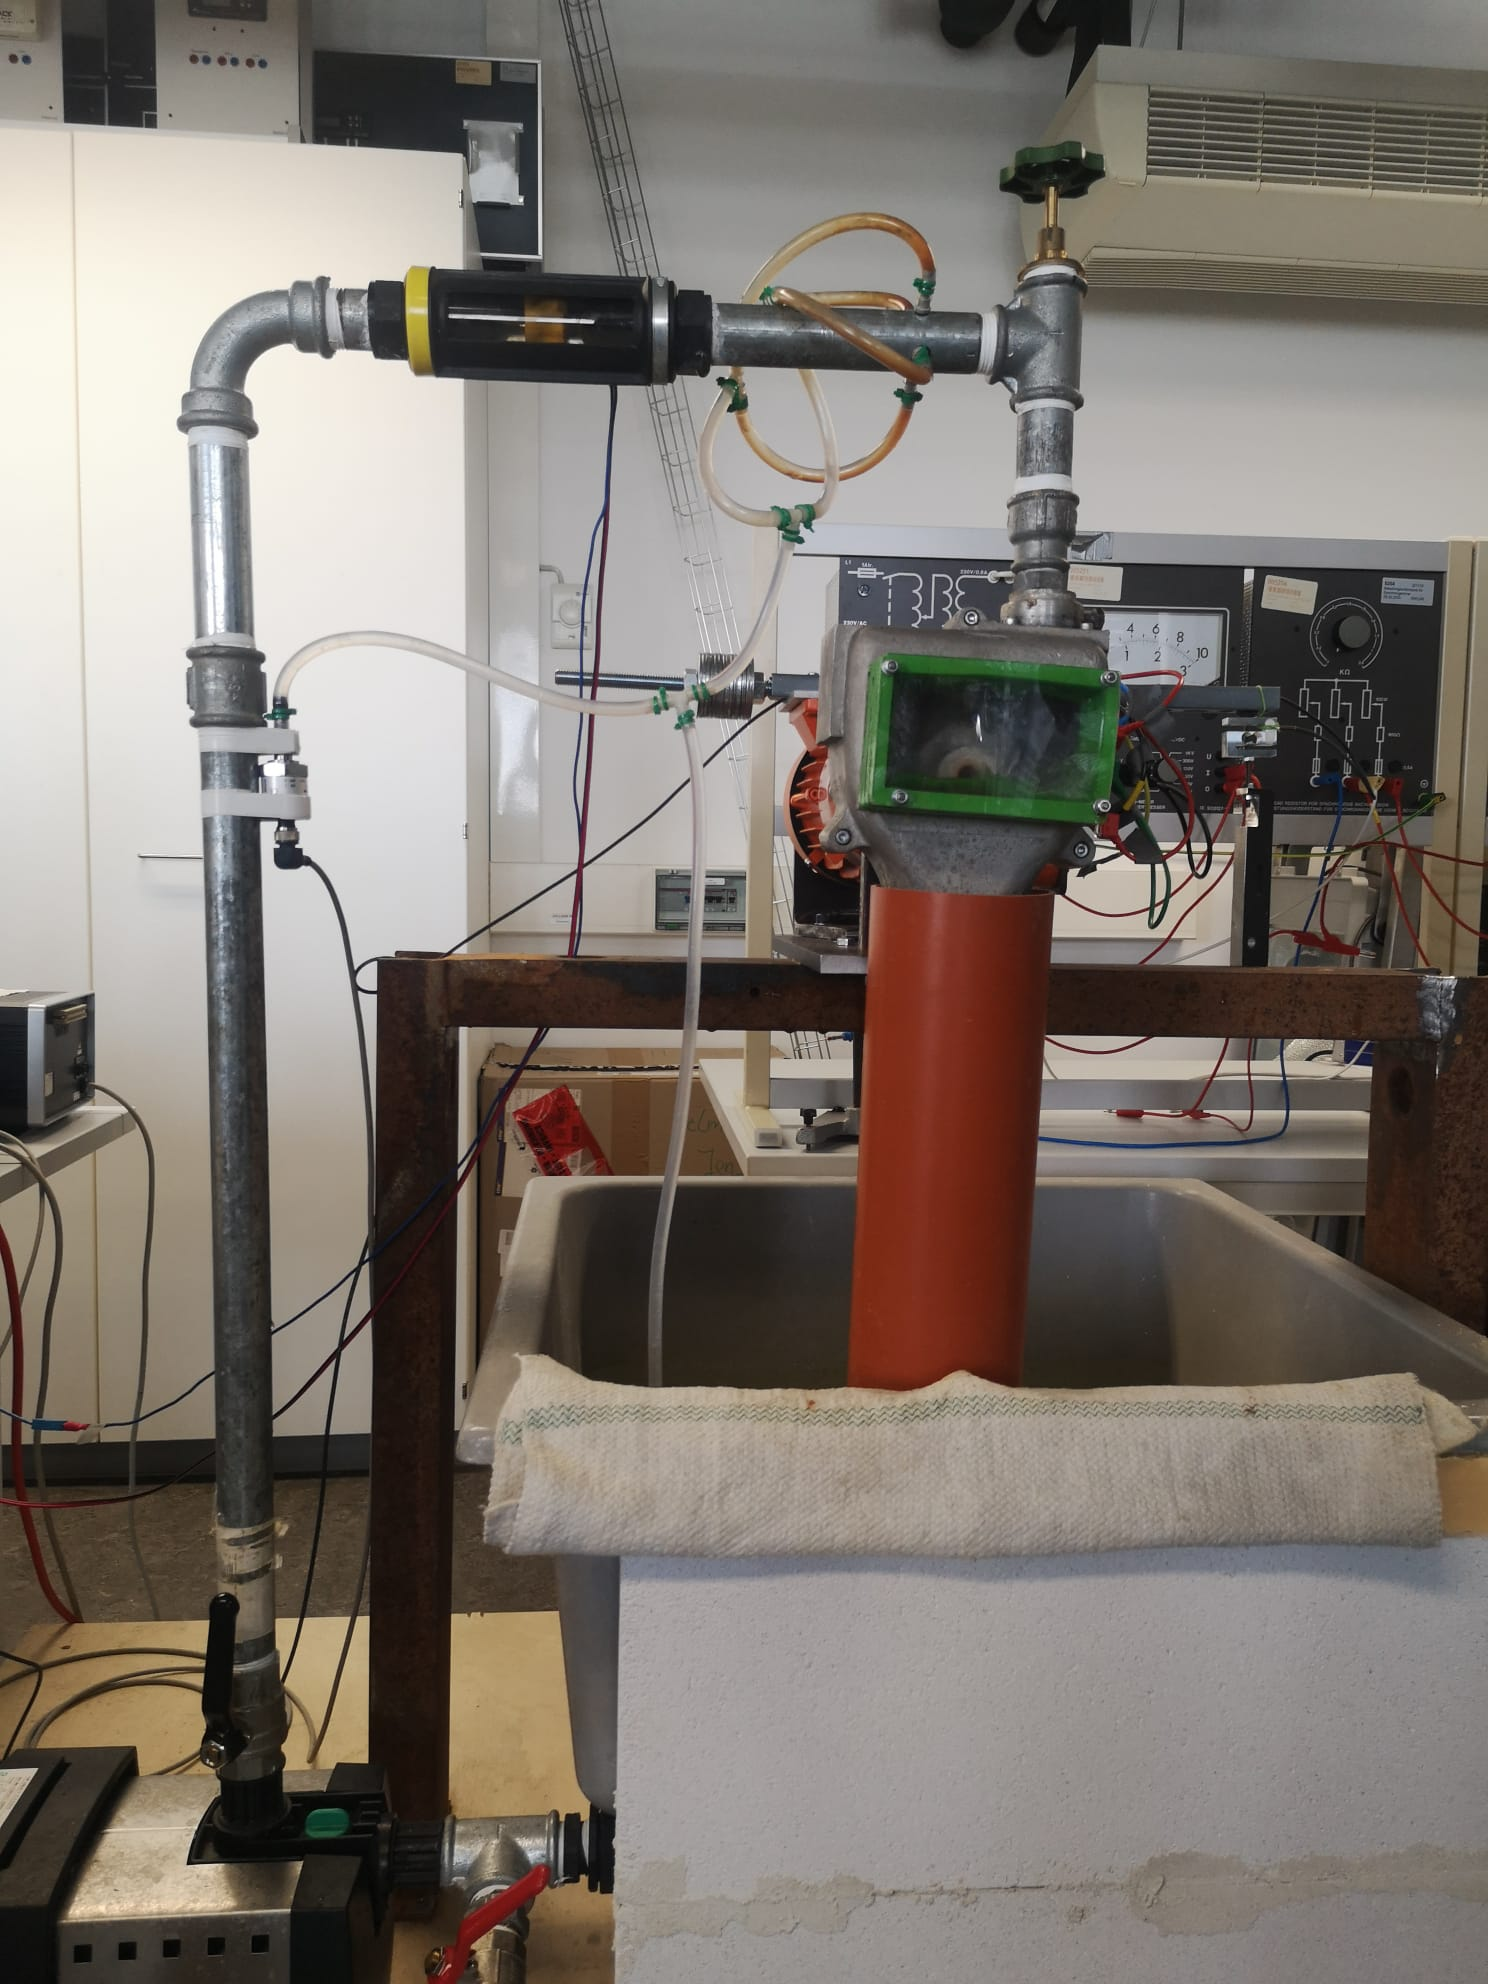
\includegraphics[scale=0.15]{Abbildungen/Aufbau Pelton.jpeg}
    \caption{Versuchsaufbau im Stillstand}
    \label{fig:Aufbau_Stillstand}
\end{figure}

An die Achse der Pelton-Turbine ist zusätzlich ein fremderregter Synchrongenerator mit einstellbarer Last gekoppelt.
Die Drehzahl der Turbine wird mit einem Handmessgerät auf der verlängerten Generatorwelle und die mechanische Belastung direkt am Generator mittels eines Kraftsensors gemessen.\\
Als Drehzahlmessgerät  wird der \textit{VOLTCRAFT DT-10L} und als Kraftsensor der \textit{ME-Meßsysteme KD40S} verwendet.
Die Draufsicht auf die Kopplung und den Synchrongenerator ist in \autoref{fig:Synchrongenerator} dargestellt.\\

\begin{figure}[H]
    \centering
    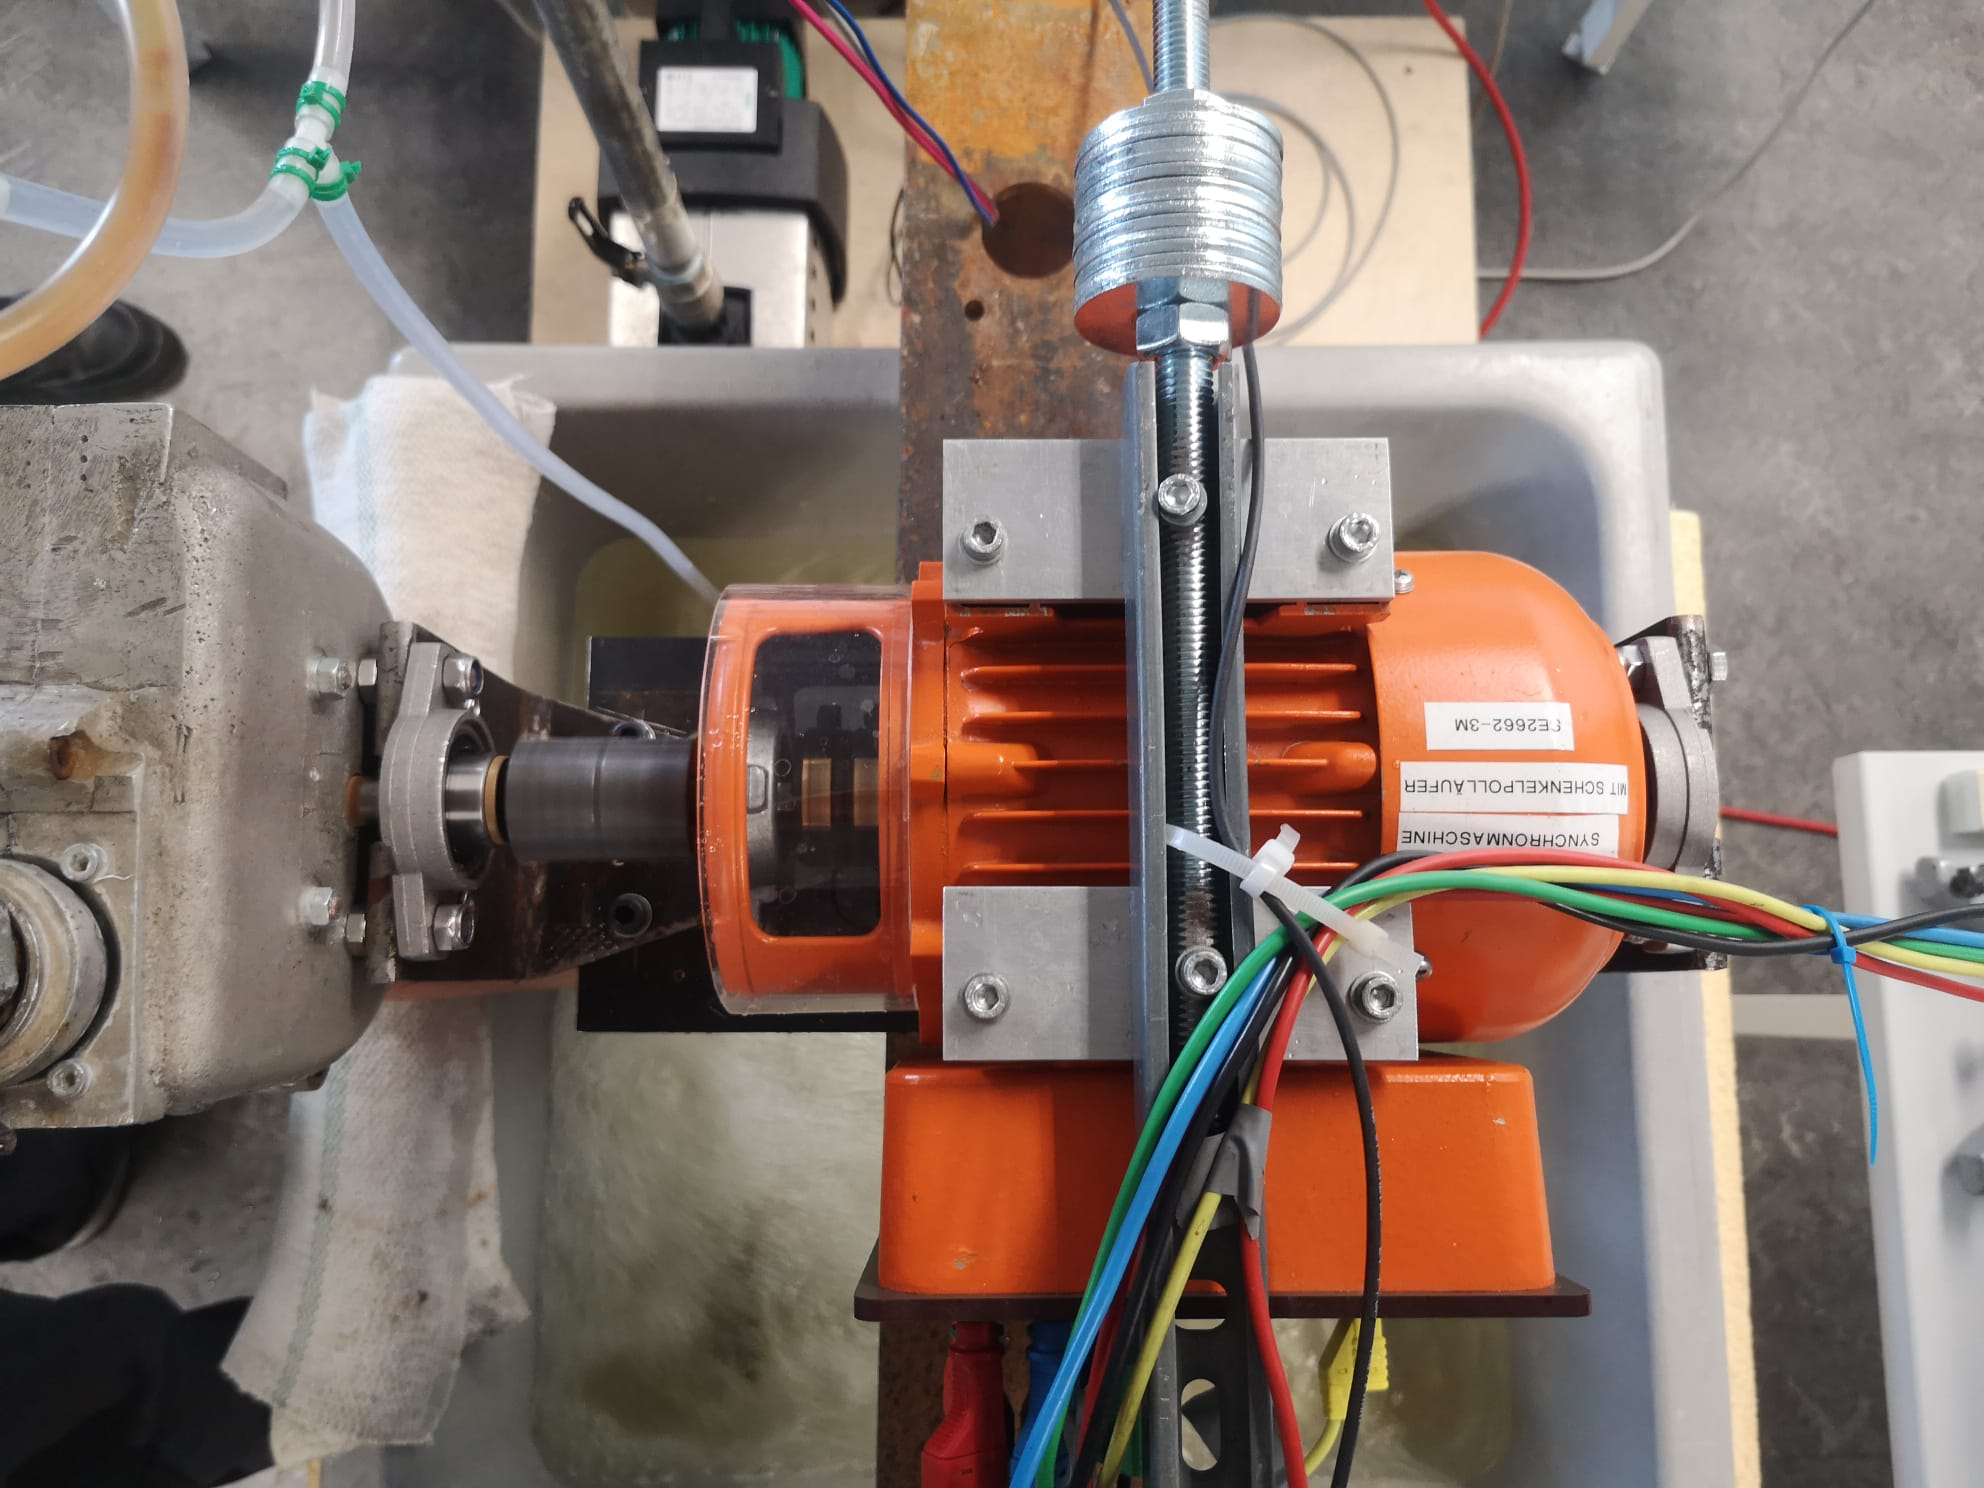
\includegraphics[width=0.5\textwidth]{Abbildungen/Generator.jpeg}
    \caption{Synchrongenerator}
    \label{fig:Synchrongenerator}
\end{figure}

Um den Erregerstrom des Synchrongenerators einstellen und anzeigen lassen zu können ist der Generator in einer Sternschaltung an eine Schalttafel angeschlossen.
An der Schalttafel kann auch der Lastwiderstand eingestellt werden.\\
Zusätzlich werden zwei Multimeter angeschlossen um den Phasenstrom, sowie die Leiterspannung messen zu können.\\
Der gesamte Aufbau der Schalttafel inklusive Multimeter ist in \autoref{fig:Schalttafel} zu sehen.

\begin{figure}[!ht]
    \centering
    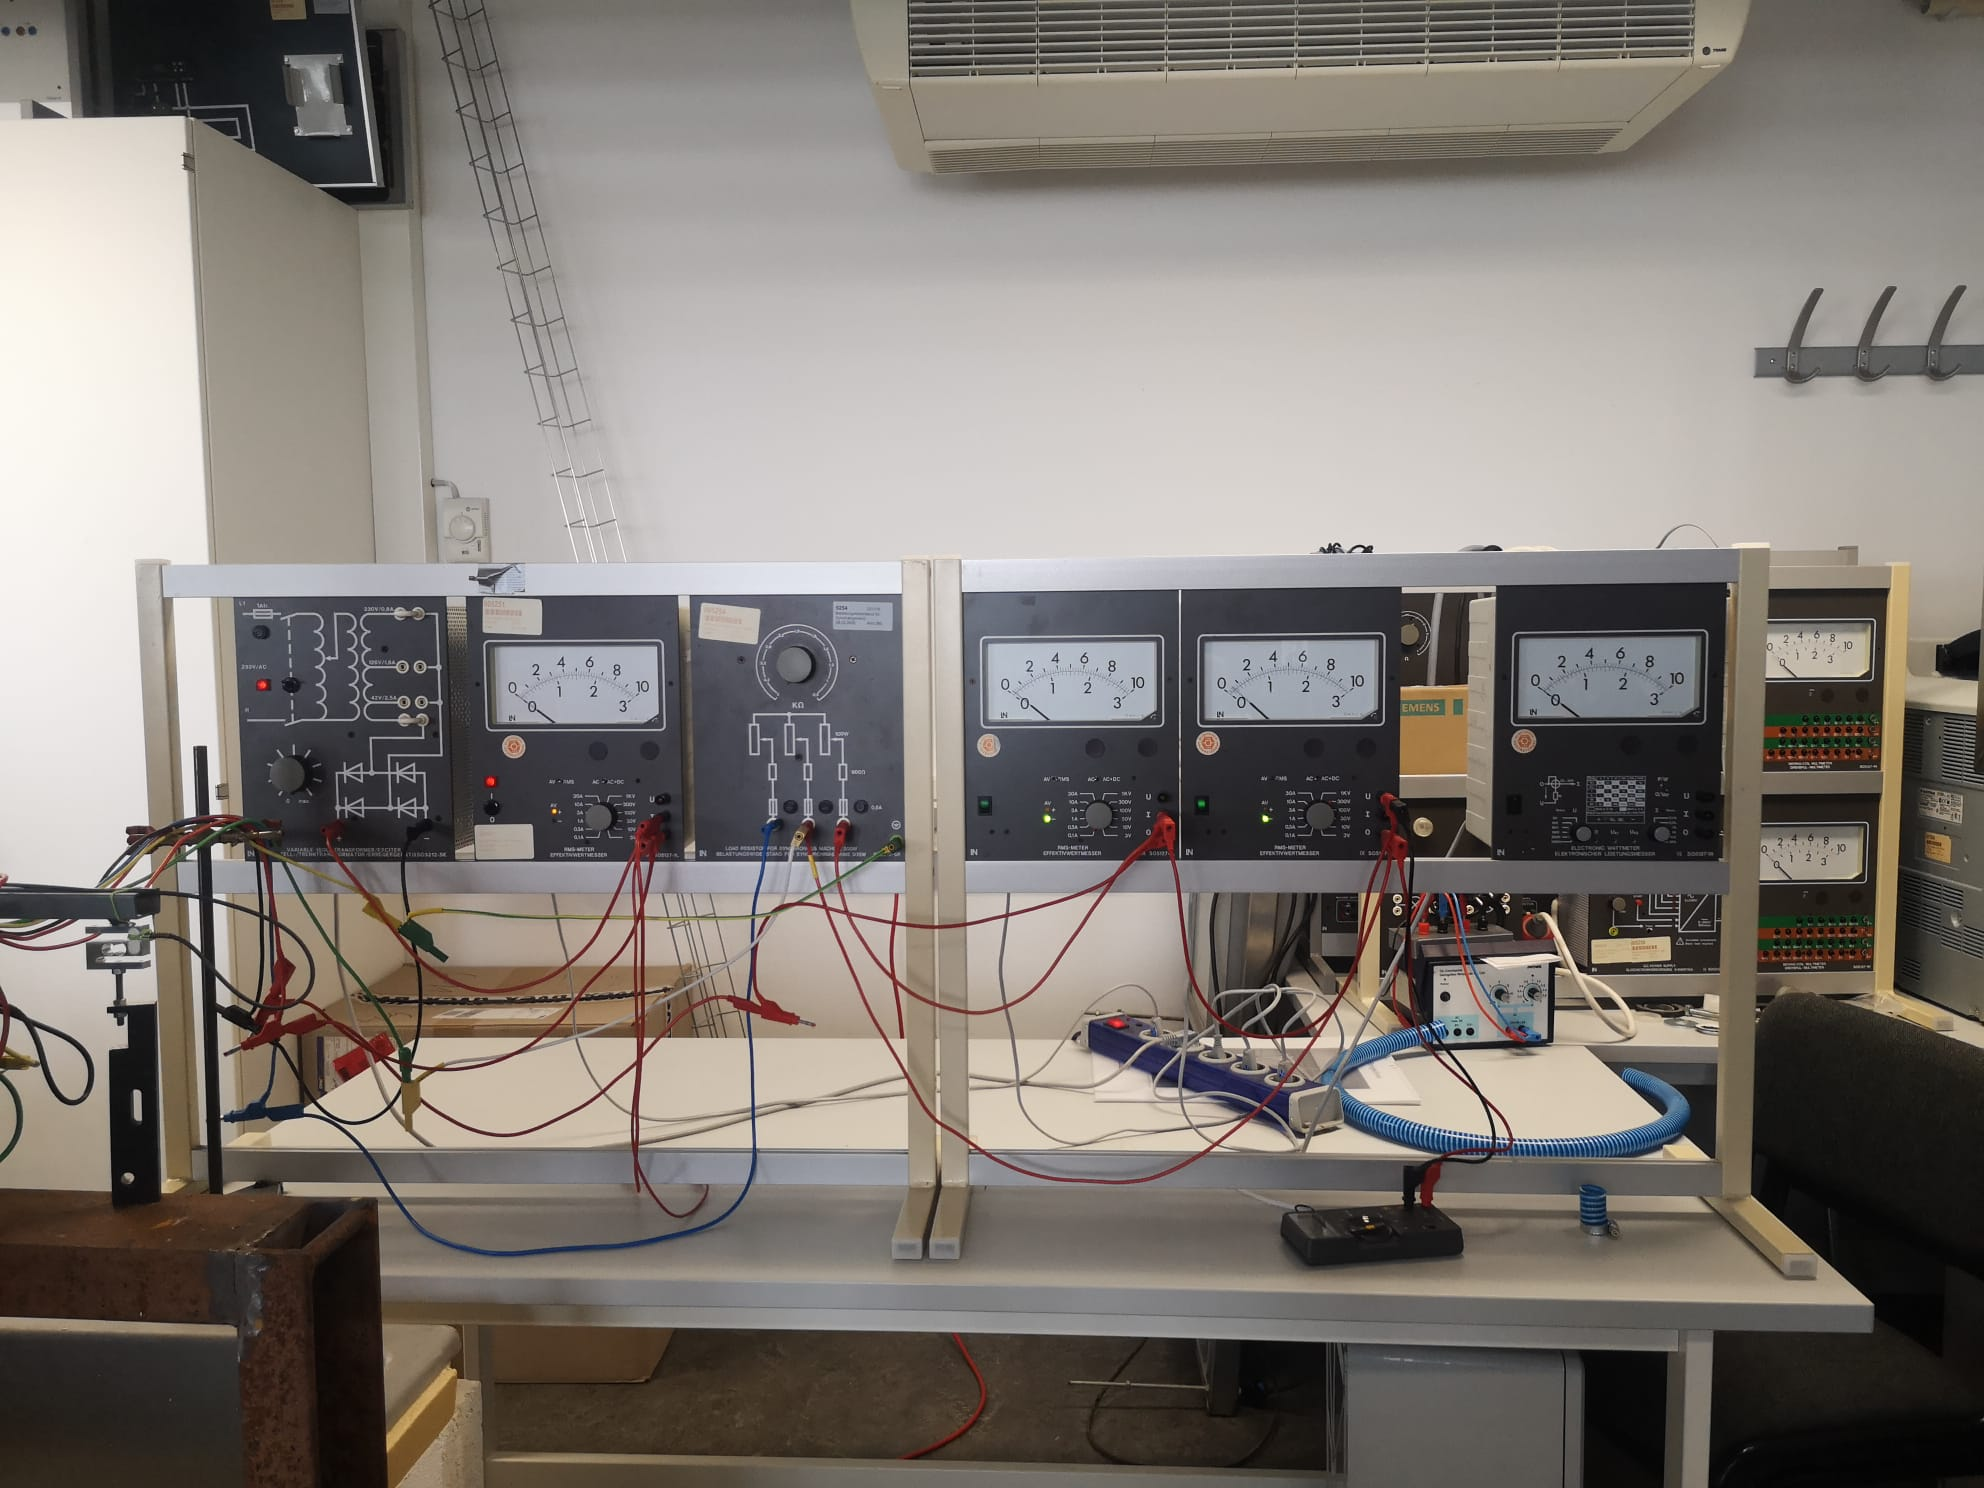
\includegraphics[width=0.5\textwidth]{Abbildungen/Schalttafel.jpeg}
    \caption{Schalttafel}
    \label{fig:Schalttafel}
\end{figure}